% jepctl: a local runtime for joint-embedding predictive architectures.
% arXiv-ready source. Complies with arXiv format requirements:
%   - no line numbers, single spaced, 11pt type, 1 inch margins
%   - no watermarks, no highlighted text, no embedded JavaScript, no animated figures
% Build:  pdflatex jepctl && bibtex jepctl && pdflatex jepctl && pdflatex jepctl
%
% TODO(author): complete the surname and affiliation on the \author line below
% before submitting; arXiv shows this block verbatim on the abstract page.

\documentclass[11pt,onecolumn]{article}

\usepackage[margin=1in]{geometry}
\usepackage[T1]{fontenc}
\usepackage[utf8]{inputenc}
\usepackage{lmodern}
\usepackage{amsmath,amssymb}
\usepackage{graphicx}
\usepackage{array}
\usepackage{booktabs}
\usepackage{microtype}
\usepackage{xcolor}
\definecolor{jepctlpanel}{HTML}{F0F7FE}
\usepackage{tikz}
\usetikzlibrary{positioning,arrows.meta,fit,backgrounds}
\usepackage[hidelinks]{hyperref}
\usepackage{url}

\newcommand{\jepctl}{\texttt{jepctl}}
\newcommand{\code}[1]{\texttt{#1}}

\title{\jepctl{}: A Local Runtime for Joint-Embedding Predictive\\ Architectures, with Few-Shot Perception, an Online\\ Latent World Model, and Robot Control}

% TODO(author): replace with your full name and affiliation.
\author{Younss\\
  Independent researcher\\
  \texttt{younssiga@gmail.com}}

\date{\today}

\begin{document}
\maketitle

\begin{abstract}
\sloppy
Joint-Embedding Predictive Architectures (JEPAs) learn by predicting representations
rather than pixels, and a growing body of work shows that the resulting latent spaces
support recognition, anomaly detection, and control. That capability is largely
confined to research code: running a JEPA encoder on a laptop, against a live camera or
microphone, and wiring it to an application still requires assembling a Python stack by
hand. We present \jepctl{}, a single-binary local runtime that makes JEPA-style
encoders operational the way \code{ollama} made local language models operational. It
loads published checkpoints with strict, auditable weight coverage; exposes embeddings
over a REST and SSE API and a command line; and ships four worked applications that use
only latent-space operations: (i) few-shot visual and audio recognition from a handful
of captures, with a per-patch divergence map that localises the deviation; (ii) an
online latent world model over the live camera that predicts the next embedding and
reports its prediction error as a surprise signal, following the design of LeWorldModel
\cite{lewm2026}; (iii) a robot arm driven either by continuous posture mirroring or by
minimising a latent energy toward a goal image, with no trajectory programming and no
reward; and (iv) a multimodal companion that fuses vision and audio locally at
\mbox{30\,Hz}. Everything runs on device: no cloud, no transcription model, and no
object detector. We report single-machine measurements on an Apple M5 Pro, including
full checkpoint coverage for six published encoders, per-frame latencies of 12--46\,ms
for a DINOv2-S front end, and a peak resident set of 1.98\,GB for a V-JEPA~2 clip
forward after removing an autograd-graph retention bug. We also state plainly what this
class of model does not provide: it is not generative and it does not produce metric
depth. \jepctl{} is Apache-2.0 licensed and available at
\url{https://github.com/younss/jepctl}.
\end{abstract}

\section{Introduction}

A predictive model of the world is useful only if something can run it. The JEPA line of
work \cite{lecun2022path,ijepa2023,vjepa2_2025} argues that an agent should learn by
predicting \emph{representations} of what it has not yet seen, rather than reconstructing
pixels, and recent results extend that principle to end-to-end training from raw pixels
\cite{lewm2026} and to domains far from vision \cite{jepaanything2026}. What has not kept
pace is the path from a published checkpoint to a working local system. Language models
crossed that gap when single-binary runtimes made ``pull a model, run it, call an API''
a one-line operation \cite{ollama}. Representation learning has no equivalent: a
practitioner who wants to use I-JEPA or V-JEPA~2 against their own webcam assembles a
Python environment, writes their own preprocessing, and discovers only at inference time
whether the checkpoint layout they downloaded matches the architecture they built.

\begin{figure}[t]
\centering
% The source artwork carries three garbled strings from the image generator: the mock
% terminal, "vo:" for "via:", and "Train to tcrinring". They are covered here with vector
% text so the figure is legible and correct; the artwork itself is unchanged.
\begin{tikzpicture}[inner sep=0pt, outer sep=0pt]
  \node[anchor=south west] (img) {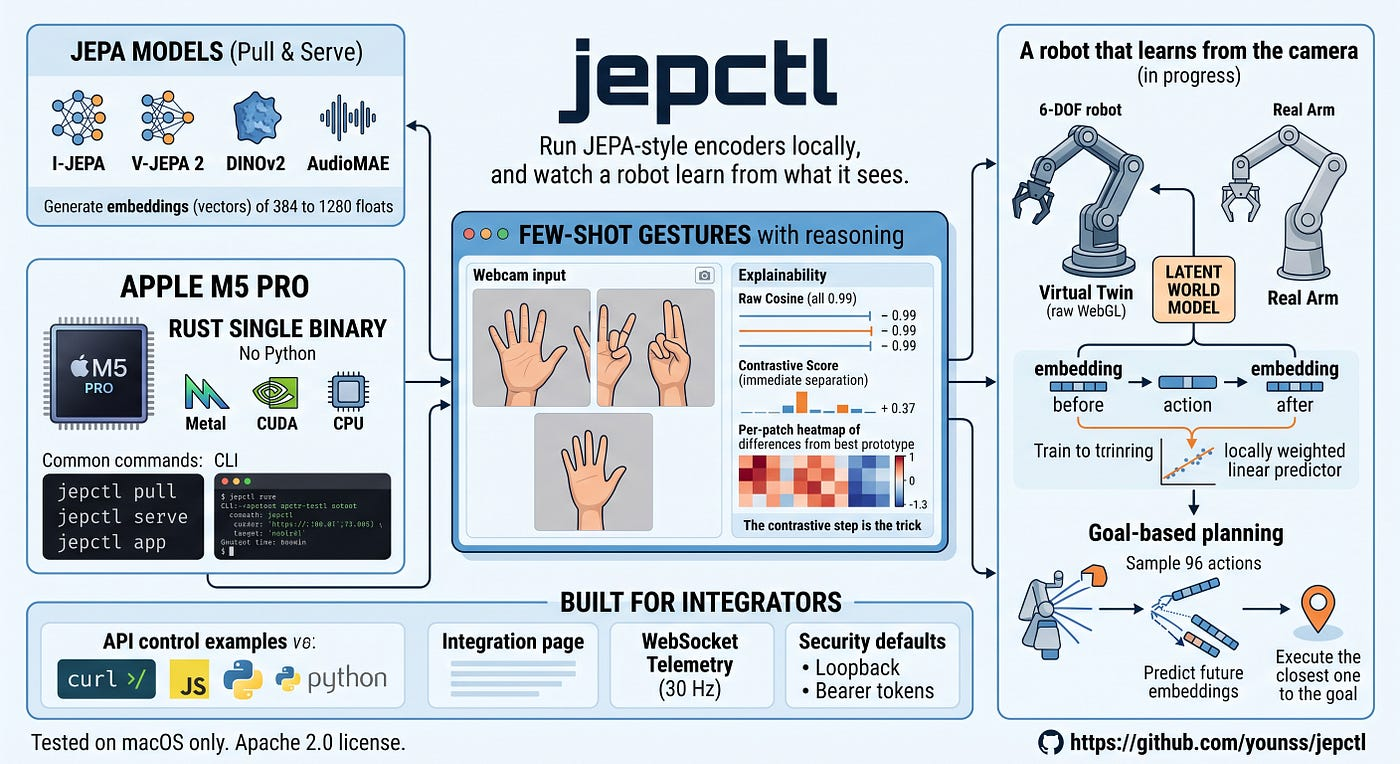
\includegraphics[width=\textwidth]{figures/jepa-overview.jpg}};
  \begin{scope}[x={(img.south east)}, y={(img.north west)}, font=\sffamily]
    % (1) Mock terminal: repaint the panel and typeset real jepctl output.
    \fill[rounded corners=1.2pt, black!92] (0.1500,0.2660) rectangle (0.2815,0.3780);
    \fill[rounded corners=1.2pt, black!75] (0.1500,0.3590) rectangle (0.2815,0.3780);
    \fill[black!92] (0.1500,0.3590) rectangle (0.2815,0.3650);
    \fill[red!70!black]    (0.1560,0.3690) circle (0.0028);
    \fill[yellow!75!black] (0.1625,0.3690) circle (0.0028);
    \fill[green!60!black]  (0.1690,0.3690) circle (0.0028);
    \node[anchor=north west, text=white, font=\ttfamily\fontsize{3.4}{4.2}\selectfont,
          align=left] at (0.1545,0.3545)
      {\$ jepctl serve\\[0.7pt]
       \textcolor{green!60!white}{INFO} Metal backend ready\\[0.7pt]
       \textcolor{green!60!white}{INFO} dinov2-small 221/221\\[0.7pt]
       \textcolor{green!60!white}{INFO} listening 127.0.0.1:11435\\[0.7pt]
       \$ \rule{1.1pt}{2.6pt}};
    % (2) "vo:" -> "via:"
    \fill[white] (0.2075,0.1450) rectangle (0.2300,0.1760);
    \node[anchor=west, font=\sffamily\itshape\fontsize{6.4}{7.5}\selectfont, text=black!85]
      at (0.2085,0.1600) {via:};
    % (3) "Train to tcrinring" -> a correct label
    \fill[rounded corners=1pt, jepctlpanel] (0.7330,0.3900) rectangle (0.8320,0.4300);
    \node[anchor=west, font=\sffamily\fontsize{5.6}{6.6}\selectfont, text=black!85,
          align=left] at (0.7355,0.4100) {Fit on observed\\ transitions};
  \end{scope}
\end{tikzpicture}
\caption{Overview of \jepctl{}. Left: catalogued JEPA-style encoders (I-JEPA, V-JEPA~2,
DINOv2, AudioMAE) producing embeddings of 384 to 1280 dimensions, served by a single Rust
binary with Metal, CUDA, or CPU backends and a small command line. Centre: few-shot
recognition with its reasoning exposed, including the raw cosine scores, the contrastive
score that separates otherwise near-identical classes, and the per-patch difference map.
Right: the camera-driven robot loop, in which embeddings before and after an action train
a locally weighted linear predictor that is then used to plan by sampling candidate
actions and executing the one predicted to land closest to the goal. Bottom: the
integration surface and the security defaults. Figure by the author.}
\label{fig:overview}
\end{figure}

\jepctl{} is that missing runtime. It is a single Rust binary with no Python dependency
that (a) downloads and loads JEPA-style checkpoints with an explicit, auditable report of
how many tensors were covered, (b) serves embeddings over HTTP, a live SSE stream, and a
command line, and (c) ships a desktop testbench in which four applications are built
entirely out of latent-space operations.

The contribution of this paper is not a new architecture or a new training objective. It
is a system, and three claims about it:

\begin{enumerate}
  \item \textbf{Operational honesty is a feature, not an implementation detail.} Loading
  a checkpoint partially yields a model that still returns vectors of the right shape and
  is therefore indistinguishable from a working one at the API level. \jepctl{} refuses
  to serve such a model and reports coverage explicitly (Section~\ref{sec:weights}).
  \item \textbf{A frozen encoder plus a small online predictor is enough to demonstrate
  the world-model loop on a laptop.} We follow the structure of LeWorldModel
  \cite{lewm2026} --- predict the next embedding, read the prediction error as surprise
  --- but freeze the encoder and fit the predictor online on the live stream, which makes
  the loop observable in seconds without a training run (Section~\ref{sec:world}).
  \item \textbf{Several economically interesting behaviours need no training at all.}
  Few-shot industrial inspection, skeleton-free teleoperation, and reward-free visual goal
  reaching are all nearest-prototype or energy-minimisation queries in a pretrained latent
  space (Sections~\ref{sec:fewshot}--\ref{sec:robot}).
\end{enumerate}

\section{Background and related work}

\paragraph{Joint-embedding predictive architectures.}
A JEPA encodes an observation $o$ into a latent $z = f_\theta(o)$ and trains a predictor
to map a context latent to the latent of a target that was masked or displaced in time,
minimising a distance in embedding space rather than in pixel space
\cite{lecun2022path}. I-JEPA applies this to masked image regions \cite{ijepa2023};
V-JEPA~2 extends it to video with spatio-temporal tubelets and demonstrates planning
\cite{vjepa2_2025}. DINOv2, while trained with a different self-distillation objective,
produces patch-level features with the same practical property we rely on here: semantic
structure that is stable under nuisance variation \cite{dinov2_2023}.

\paragraph{LeWorldModel.}
Maes et al.\ \cite{lewm2026} address the central fragility of JEPA training --- collapse
to a constant representation --- with a two-term objective: a mean-squared next-embedding
prediction loss, and SIGReg, a regulariser that projects embeddings onto random
directions and applies a normality test to each one-dimensional projection, pushing the
latent distribution toward an isotropic Gaussian. The result trains stably end to end from
pixels without stop-gradients, exponential moving averages, or a pretrained encoder,
with 15M parameters on a single GPU. Two of their findings are directly load-bearing for
this work. First, the predictor is autoregressive in latent space: $z_{t+1}$ is predicted
from $z_t$ and the action $a_t$. Second, the resulting prediction error is a usable
\emph{surprise} signal: the model reliably flags physically implausible events. Our World
module (Section~\ref{sec:world}) implements that loop with a frozen encoder, and our robot
goal-reaching module (Section~\ref{sec:robot}) plans by rolling out a learned latent
transition model, in the spirit of their cross-entropy-method planner \cite{cem2004}.

\paragraph{JEPA-Anything.}
Cui et al.\ \cite{jepaanything2026} argue the complementary point: that the JEPA principle
is domain-agnostic. Their orthogonal predictive factorization decomposes latent targets
into complementary factors learned through dedicated pathways and recombined in a shared
predictive design, validated across vision, biology, clinical trajectories, control,
molecular dynamics, physical fields, and weather. Their result motivates a runtime whose
abstractions are modality-agnostic: \jepctl{} treats an image, a video clip, and an audio
spectrogram as the same object --- an input that becomes an embedding --- and its
few-shot matcher, its world model, and its control loops are written against embeddings,
not against pixels. We do not implement OPF; we take from that work the design constraint
that nothing in the runtime above the encoder should assume a modality.

\paragraph{What this is not.}
JEPA encoders are not generative. They do not decode a latent back to pixels, and they do
not estimate metric depth. Throughout this paper, and in the software's own interface, we
are explicit about that boundary; Section~\ref{sec:limits} states it as a limitation
rather than hiding it behind a visualisation.

\section{System design}

\jepctl{} is written in Rust and builds to one binary. Inference uses \code{candle}
\cite{candle} with Metal, CUDA, or multi-threaded CPU backends selected at runtime. The
HTTP layer is \code{axum}; the desktop testbench is a native window hosting a
dependency-free web UI. Figure~\ref{fig:overview} gives the overall picture and
Figure~\ref{fig:arch} the dataflow.

\begin{figure}[t]
\centering
\resizebox{\textwidth}{!}{%
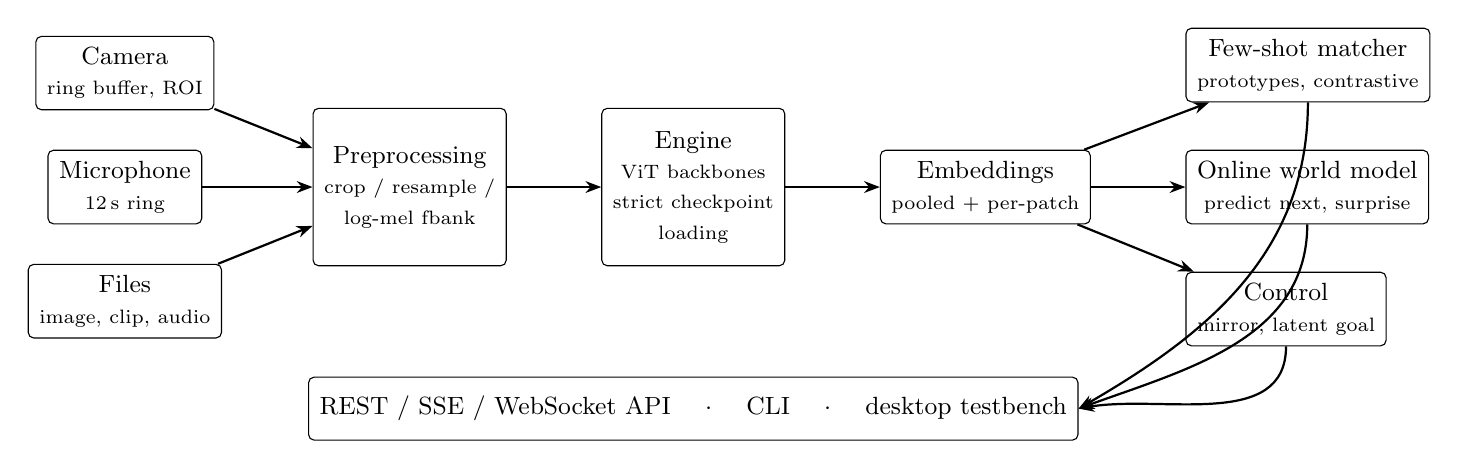
\begin{tikzpicture}[
  node distance=5mm,
  box/.style={draw, rounded corners=2pt, align=center, font=\small, inner sep=4pt, minimum height=8mm},
  grp/.style={draw, dashed, rounded corners=3pt, inner sep=6pt},
  arr/.style={-{Stealth[length=2mm]}, thick}
]
\node[box] (cam) {Camera\\\scriptsize ring buffer, ROI};
\node[box, below=of cam] (mic) {Microphone\\\scriptsize 12\,s ring};
\node[box, below=of mic] (files) {Files\\\scriptsize image, clip, audio};

\node[box, right=14mm of mic, minimum height=20mm] (pre) {Preprocessing\\\scriptsize crop / resample /\\\scriptsize log-mel fbank};

\node[box, right=12mm of pre, minimum height=20mm] (eng) {Engine\\\scriptsize ViT backbones\\\scriptsize strict checkpoint\\\scriptsize loading};

\node[box, right=12mm of eng] (emb) {Embeddings\\\scriptsize pooled $+$ per-patch};

\node[box, above right=6mm and 12mm of emb] (fs) {Few-shot matcher\\\scriptsize prototypes, contrastive};
\node[box, right=12mm of emb] (wm) {Online world model\\\scriptsize predict next, surprise};
\node[box, below right=6mm and 12mm of emb] (ctl) {Control\\\scriptsize mirror, latent goal};

\node[box, below=14mm of eng] (api) {REST / SSE / WebSocket API \quad $\cdot$ \quad CLI \quad $\cdot$ \quad desktop testbench};

\draw[arr] (cam) -- (pre);
\draw[arr] (mic) -- (pre);
\draw[arr] (files) -- (pre);
\draw[arr] (pre) -- (eng);
\draw[arr] (eng) -- (emb);
\draw[arr] (emb) -- (fs);
\draw[arr] (emb) -- (wm);
\draw[arr] (emb) -- (ctl);
\draw[arr] (fs.south) to[out=-90,in=30] (api.east);
\draw[arr] (wm.south) to[out=-90,in=20] (api.east);
\draw[arr] (ctl.south) to[out=-90,in=10] (api.east);
\end{tikzpicture}}
\caption{\jepctl{} architecture. Every module above the encoder operates on embeddings
only; none of them reads pixels. The same path serves the command line, the HTTP API, and
the desktop testbench.}
\label{fig:arch}
\end{figure}

\subsection{Strict checkpoint loading}
\label{sec:weights}

A partially loaded Vision Transformer \cite{vit2021} is a silent failure: the forward pass succeeds, the
output has the advertised dimension, and every downstream metric is meaningless. \jepctl{}
therefore maps every parameter of the constructed backbone against the checkpoint,
trying the naming conventions of Hugging Face ViT/I-JEPA, Hugging Face DINOv2, Hugging
Face V-JEPA~2, and timm-style fused QKV, and reshaping tensors whose element count matches
(for instance a \code{Conv3d} patch kernel feeding a linear tubelet embedding). It then
returns a coverage report. A model whose coverage is below 100\,\% is refused with HTTP
422 rather than served. Positional embeddings are adapted separately: the CLS row is
sliced or synthesised as required, and the patch grid is resampled bicubically when the
checkpoint resolution differs from the configured one.

Weights are read from \code{safetensors} \cite{safetensors}, which is parsed and
memory-mapped but never executed; this removes the arbitrary-code-execution surface of
pickle-based checkpoints. Table~\ref{tab:weights} lists the coverage we obtain for the
catalogued encoders.

\begin{table}[t]
\centering
\small
\begin{tabular}{llrr}
\toprule
Checkpoint & Family & Dim & Coverage \\
\midrule
\code{facebook/ijepa\_vith14\_1k}                      & I-JEPA ViT-H/14   & 1280 & 516/516 \\
\code{facebook/dinov2-small}                           & DINOv2 ViT-S/14   & 384  & 221/221 \\
\code{facebook/vjepa2-vitl-fpc64-256}                  & V-JEPA~2 ViT-L    & 1024 & 388/388 \\
\code{google/vit-base-patch16-224}                     & ViT-B/16          & 768  & 197/197 \\
timm ViT-B/16 (fused QKV)                              & ViT-B/16          & 768  & 197/197 \\
{\footnotesize\code{gaunernst/vit\_base\_patch16\_1024\_128.audiomae\_as2m}} & AudioMAE ViT-B & 768 & 197/197 \\
\bottomrule
\end{tabular}
\caption{Checkpoint coverage reported by \jepctl{} for the catalogued encoders. Coverage
is the number of backbone parameters populated from the checkpoint over the number the
architecture declares; anything below 100\,\% is refused at load time.}
\label{tab:weights}
\end{table}

\subsection{Modality-agnostic input path}

Images are centre-cropped and resized to the model input with the normalisation declared
by the manifest (ImageNet or Inception statistics). Video clips are decoded natively for
GIF and animated WebP and through an external \code{ffmpeg} binary for MP4/WebM, then
uniformly sub-sampled to the clip length the model expects; image models embed each
sampled frame and average. Audio is down-mixed to mono, resampled to 16\,kHz, and turned
into a Kaldi-style log-mel filterbank of $1024 \times 128$ for the AudioMAE front end
\cite{audiomae2022}. Because that encoder's CLS token was never trained as a summary, the
manifest selects mean pooling; using CLS yields near-identical vectors for every input,
which is exactly the kind of silent failure the coverage report is designed to prevent.

\subsection{Deployment posture}

The daemon binds \code{127.0.0.1} by default and can be switched to all interfaces from a
settings toggle, in which case authentication is mandatory. Bearer tokens are stored as
SHA-256 digests and compared in constant time; no CORS headers are emitted by default, so
a web page open in the user's browser cannot read camera frames or embeddings. Decoders
are bounded (8192\,px per side, 256\,MB of decoder allocation, 512 frames or 256 million
pixels per animation) so that a decompression bomb is refused before it is allocated.

\section{Few-shot perception in latent space}
\label{sec:fewshot}

The first application registers a small number of reference embeddings per class and
classifies by similarity. Let $\{z_i^{(c)}\}$ be the $\ell_2$-normalised embeddings
captured for class $c$ and $p_c$ their normalised mean. For a query $z$, a naive matcher
scores $\cos(z, p_c)$. That score is dominated by whatever the classes share --- the room,
the lighting, the operator's torso. \jepctl{} therefore also computes a contrastive score
in the centroid-removed subspace: with $\bar p = \frac{1}{C}\sum_c p_c$, it scores
$\cos(z - \bar p,\; p_c - \bar p)$, and reports a blend
$s_c = 0.35\,\cos(z,p_c) + 0.65\,\cos(z-\bar p, p_c - \bar p)$, gated by a threshold and a
minimum lead over the runner-up. A dedicated \emph{neutral} class absorbs frames in which
nothing intentional is present, which is what prevents an empty scene from being forced
into the nearest class.

\paragraph{Localising the deviation.}
Because the encoder emits one vector per patch, the same machinery localises \emph{where}
a query departs from its prototype: the per-patch distance to the best-ranked class's
patch prototype, arranged on the $16\times16$ ViT grid, is a divergence map. In the
industrial-inspection scenario shipped with the tool --- a bottle, capped or not --- two
short captures are enough to separate the two states, and the divergence map concentrates
on the neck. Nothing was ever trained to look for a cap; the localisation is a consequence
of patch-level semantics. This is the property that makes the approach economically
interesting: the classical alternative requires a labelled dataset and a training run per
defect class.

\paragraph{Why latent space rather than pixel differencing.}
Glass and plastic produce specular highlights that move with the operator and the ambient
light. Pixel differencing responds strongly to those high-frequency luminance changes; the
patch embeddings we use are comparatively stable under them, because the pretraining
objective rewards representations that are predictable across nuisance variation. We report
this as an observed qualitative behaviour of the shipped scenario, not as a quantitative
robustness claim.

\section{An online latent world model over the live camera}
\label{sec:world}

The World module implements the LeWorldModel loop \cite{lewm2026} with one deliberate
substitution: the encoder is frozen (any catalogued JEPA encoder) and only the predictor
is fit, online, on the live stream. This trades the representation-learning contribution
of \cite{lewm2026} --- which their SIGReg term exists to protect --- for something a user
can watch converge in seconds on a laptop, with no training run and no checkpoint to
distribute. Figure~\ref{fig:loop} shows the loop.

\begin{figure}[t]
\centering
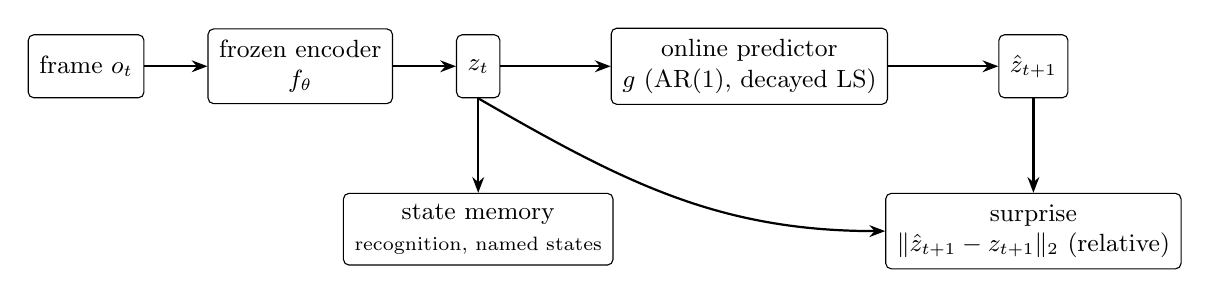
\begin{tikzpicture}[
  node distance=8mm,
  box/.style={draw, rounded corners=2pt, align=center, font=\small, inner sep=4pt, minimum height=8mm},
  arr/.style={-{Stealth[length=2mm]}, thick}
]
\node[box] (o) {frame $o_t$};
\node[box, right=of o] (f) {frozen encoder\\$f_\theta$};
\node[box, right=of f] (z) {$z_t$};
\node[box, right=14mm of z] (p) {online predictor\\$g$ (AR(1), decayed LS)};
\node[box, right=14mm of p] (zh) {$\hat z_{t+1}$};
\node[box, below=12mm of zh] (err) {surprise\\$\|\hat z_{t+1} - z_{t+1}\|_2$ (relative)};
\node[box, below=12mm of z] (mem) {state memory\\\scriptsize recognition, named states};

\draw[arr] (o) -- (f);
\draw[arr] (f) -- (z);
\draw[arr] (z) -- (p);
\draw[arr] (p) -- (zh);
\draw[arr] (zh) -- (err);
\draw[arr] (z) -- (mem);
\draw[arr] (z.south) to[out=-30,in=180] (err.west);
\end{tikzpicture}
\caption{The World loop. The encoder is frozen; the predictor is fit online from the
stream. The prediction error of the previous step, normalised by the recent typical error,
is the surprise signal used for anomaly detection, following \cite{lewm2026}.}
\label{fig:loop}
\end{figure}

\paragraph{Predictor.}
The pooled embedding is projected onto a fixed random basis of dimension $K=48$; by the
Johnson--Lindenstrauss lemma \cite{jl1984} this preserves distances well enough for the
error statistic we need while keeping the online fit cheap and stable. In that space a
per-dimension first-order autoregression $x_{t+1} = a \odot x_t + c$ is fit by decayed
least squares (decay $0.97$), falling back to persistence until enough transitions have
accumulated.

\paragraph{Surprise.}
Let $e_t = \|\hat z_t - z_t\|_2$ be the error of the prediction made at $t-1$, and
$\bar e$ an exponentially weighted estimate of the recent typical error. The reported
surprise is $\mathrm{clip}\big((e_t/\bar e - 1)/1.5,\,0,\,1\big)$, so that a scene the
model tracks well sits near zero and a genuine deviation spikes. This is the
operationalisation of the surprise evaluation in \cite{lewm2026}: prediction error in
latent space, not in pixel space, is what flags the implausible event. Per patch, the same
comparison against a constant-velocity prediction $2z_t - z_{t-1}$ yields a spatial
surprise map, which the interface renders as a glow on the diverging region and which
drives a configurable alarm with a timestamped, spatially localised incident log.

\paragraph{Recognition and named states.}
A bounded memory of normalised pooled embeddings gives a recognition score (nearest
neighbour by cosine), and novel states are appended, so the system reports whether the
current view is familiar. Users may additionally save named reference states (``empty
desk'', ``full shelf''), after which the module reports which one it sees or flags the view
as unknown.

\paragraph{Rendering the perception, honestly.}
The reconstruction shown to the user maps the live frame onto a surface whose relief is
derived from the semantic distance of each patch to a background prototype (the mean of
the patches whose distance to the frame centroid is below the median). A smoothstep
transfer keeps the background flat and extrudes only the foreground, and the patch grid is
upsampled bicubically so silhouettes are smooth. We label this in the interface as what it
is: the real frame given shape by what the encoder perceives. It is neither a generated
image nor a metric depth map.

\section{Control without trajectories or rewards}
\label{sec:robot}

The robot module drives a 6-DoF arm with a gripper through a hardware abstraction trait
with two implementations: an in-memory backend feeding a WebGL twin, and a serial backend
speaking a Feetech STS3215 register protocol. A safety supervisor enforces per-joint
limits, a 1.5\,rad/s velocity ramp at 30\,Hz, and an emergency stop that only an
administrator can reset; with the physical backend every command is held until explicitly
approved. Two control modes are latent-space operations.

\paragraph{Mirror: teleoperation without skeleton tracking.}
The operator demonstrates a handful of postures, each associated with an arm pose. At run
time the arm does not snap to the winning class; it moves to the softmax-weighted blend of
the demonstrated poses, with weights
$w_c \propto \exp\big((s_c - \max_j s_j)/\tau\big)$, $\tau = 0.06$, candidates more than
$0.20$ below the best receiving zero weight and the blend suppressed entirely below a
score of $0.35$. Raising an arm slowly therefore sweeps the joint targets continuously
through the demonstrated poses. Unlike pose-estimation pipelines, no joint of the human
body is ever localised: the comparison is between whole-posture embeddings.

\paragraph{Visual goal reaching: energy minimisation in latent space.}
Following the planning structure of \cite{lewm2026}, the arm captures a goal embedding
$z_\star$ from the camera and then minimises
\begin{equation}
E(z, z_\star) \;=\; \frac{\lVert z - z_\star \rVert_2}{\sqrt{d}} ,
\end{equation}
where $d$ is the embedding dimension. A latent transition model is fit online from
exploration: triples $(z, a, z')$ collected while the arm babbles are used to fit a
locally weighted ridge regression $\Delta z = W[a;1]$, refit after every observation. At
each step the controller samples 96 candidate actions, predicts their outcome \emph{inside
the learned model}, executes the one with the lowest predicted energy plus exploration
noise, observes the real result, and learns from it. Until enough transitions exist the
policy is random, and the telemetry reports which regime is active together with predicted
versus observed energy, so the user can judge the model rather than trust it. Convergence
is declared against a noise floor measured from two observations of a static scene, and a
plateau detector reports when a single viewpoint cannot disambiguate further.

Because the virtual arm is invisible to a real camera, the observation used in simulation
is the camera frame with the twin's kinematics rendered into it over a frozen background,
so that the only thing changing between observations is the arm itself. This is a
simulation convenience and we flag it as such; with the physical backend the observation is
the raw camera frame.

\section{Multimodal companion}
\label{sec:companion}

The companion is a virtual character that fuses two frozen encoders locally. Motion
attention is computed from the centroid of the thresholded difference between consecutive
$32\times24$ grayscale thumbnails at 10\,Hz and steers the head; visual cues are matched
at roughly 3\,Hz against the gesture prototypes; audio cues are matched at roughly
1.4\,Hz from the last 1.5\,s of microphone audio, zero-padded into the AudioMAE window.
Recognised cues fire behaviours with a two-second cooldown, and postures mapped to body
poses are blended by the same softmax rule as the arm. A 30\,Hz control loop renders the
result. The point of this module is the absence of the usual machinery: there is no
transcription model, no keyword spotter, and no object detector --- a clap and a wave are
both nearest-prototype lookups over local embeddings.

\section{Measurements}
\label{sec:measure}

The numbers below were obtained on a single machine (Apple M5 Pro, 15 logical cores,
24\,GB unified memory, macOS, Metal backend) during interactive use. They characterise
this implementation on this hardware; they are not benchmarks and no baseline comparison
is claimed.

\begin{table}[t]
\centering
\small
\begin{tabular}{@{}>{\raggedright\arraybackslash}p{0.27\textwidth}>{\raggedright\arraybackslash}p{0.40\textwidth}>{\raggedright\arraybackslash}p{0.27\textwidth}@{}}
\toprule
Quantity & Setting & Observed \\
\midrule
World endpoint latency & DINOv2-S, full frame, relief and texture & 12--46\,ms per call \\
Gesture stream latency & DINOv2-S, model view & 12--15\,ms per frame \\
V-JEPA~2 clip forward & ViT-L, 16 frames at 256\,px, peak RSS & 1.98\,GB \\
Daemon under load & V-JEPA~2 loaded, SSE stream and 4 concurrent captures & 1.5\,GB peak \\
Goal reaching (simulated arm) & after $\approx$45\,s of exploration & all 6 joints within $\approx$0.1\,rad in 15--30\,s \\
Latent transition model fit & simulated arm, frozen background & fit error $\approx$0.05 \\
\bottomrule
\end{tabular}
\caption{Single-machine measurements.}
\label{tab:measure}
\end{table}

\paragraph{A memory bug worth reporting.}
Every model was originally constructed from a parameter map whose tensors were
autograd-tracked variables, because that is the natural way to copy a checkpoint into a
pre-built architecture. Inference through such tensors records a backward graph, and that
graph keeps every intermediate activation of every layer alive until the output is
dropped. Instrumenting the Metal allocator showed GPU allocation climbing linearly by
roughly 0.5\,GB per transformer layer, reaching 13.5\,GB after 24 layers for a single
V-JEPA~2 clip; with concurrent requests the process reached 36\,GB and was killed.
Rebuilding each model on detached tensors after loading --- storage is shared, so nothing
is copied --- reduced the peak resident set for one clip forward to 1.98\,GB, of which
1.2\,GB is the weights themselves. We report this because the failure mode is invisible in
a framework that assumes training: nothing is wrong except that inference is paying for a
gradient nobody will ever use.

\paragraph{Correctness practices.}
The repository contains 76 Rust unit and integration tests, including in-memory HTTP tests
of every API surface, and 4 UI tests. What has \emph{not} been done is a numerical
comparison against the reference PyTorch implementations, because the project has no
Python dependency. Implementations follow the reference code structure, including
V-JEPA~2's tiled sine/cosine rotary tables with interleaved rotation and the Kaldi Povey
window for the audio front end, and determinism and discriminativeness are checked, but a
bit-level equivalence claim would be unsupported and we do not make one.

\section{Limitations}
\label{sec:limits}

\begin{itemize}
  \item \textbf{Not generative, no metric depth.} JEPA encoders do not decode latents to
  pixels and do not estimate distance. The 3D reconstruction in the World module is the
  real camera image given relief by semantic foreground separation; calling it depth would
  be wrong.
  \item \textbf{The online predictor is weak by construction.} A per-dimension AR(1) fit in
  a 48-dimensional random projection is adequate to expose the predict-then-measure-surprise
  loop and to detect deviations, but it is not the learned predictor of \cite{lewm2026} and
  makes no claim to their control performance.
  \item \textbf{Single viewpoint.} Goal reaching can plateau at a pose that is
  view-equivalent to the goal; the system reports the plateau rather than pretending to
  converge.
  \item \textbf{Few-shot means few-shot.} Prototypes interpolate between what was
  demonstrated and do not extrapolate; recognition degrades under large changes of
  viewpoint, scale, or illumination relative to the captures.
  \item \textbf{No published Audio-JEPA checkpoint.} The audio path is complete, but the
  verified audio encoder is AudioMAE \cite{audiomae2022}; a JEPA-trained audio encoder in a
  loadable format would be a manifest entry away.
  \item \textbf{The serial robot backend is frame-tested only.} The STS3215 protocol is
  implemented from the register map and unit-tested at the frame level; it has not been run
  against physical hardware by the authors.
\end{itemize}

\section{Conclusion}

The JEPA literature has moved quickly from a training principle \cite{lecun2022path} to
stable end-to-end world models \cite{lewm2026} and to a claim of domain generality
\cite{jepaanything2026}. \jepctl{} is an attempt to close the distance between that
literature and a practitioner with a laptop and a camera: pull a checkpoint, be told
exactly how much of it loaded, and then reach for recognition, anomaly detection, or
control as operations on embeddings. The applications it ships are deliberately ordinary
--- inspect a bottle, mirror a posture, reach a pictured goal, react to a clap --- because
the interesting claim is not that any of them is novel, but that each of them costs a
handful of captures instead of a dataset, and runs entirely on the machine in front of you.

\section*{Availability}

Source code, documentation, and the model catalogue are available under the Apache-2.0
licence at \url{https://github.com/younss/jepctl}. The measurements in
Section~\ref{sec:measure} correspond to version 0.3.0.

\section*{Acknowledgements}

% TODO(author): add funding, colleagues, or remove this section before submitting.
The author thanks the maintainers of the open-source checkpoints catalogued by this tool.

\bibliographystyle{plain}
\bibliography{refs}

\end{document}
